\documentclass[fleqn,11pt]{report}

\usepackage[utf8]{inputenc}
\usepackage[T1]{fontenc}
\usepackage[francais]{babel}
%\usepackage{french} % Sommaire en début de document
\usepackage{amsmath} % Maths
\usepackage{amsfonts}	% Maths
\usepackage[top=3cm, bottom=3cm, left=3cm, right=3cm]{geometry} % Marges
\usepackage{listings} % Mise en forme du code (pour Hoare) ## À REVOIR ###
%\usepackage{ifthen} % Structures If Then Else
\usepackage{theorem} % Styles supplémentaires pour théorèmes
\usepackage{url}
\usepackage{array} % Tableaux 'typographiquement plus corrects' (?)

\usepackage{enumerate} % Changer les puces des listes d'énumération
\usepackage{setspace} % Changer les interlignes

%\usepackage{subfig} % Créer des sous-figures
\usepackage{graphicx} % Importer des images


% Redéfinition du style des caption
\makeatletter
\renewcommand{\fnum@figure}{\small\textbf{\figurename~\thefigure}}
\makeatother

% Redéfinition du style 'leo' pour les URL (police plus petite)
\makeatletter
\def\url@leostyle{%
  \@ifundefined{selectfont}{\def\UrlFont{\sf}}{\def\UrlFont{\small\ttfamily}}}
\makeatother
\urlstyle{leo}


%%% Packages temporaires %%%
%\usepackage{ulem} % Vaguelettes de soulignement
%\usepackage{soul} % Soulignements et texte barré
%\usepackage{color} % Couleurs du texte
%\newcommand{\AREVOIR}[1]{\textbf{\textcolor{red}{#1}}}
%\usepackage{algorithmic}
%\usepackage{layout}


% Définition des styles de théorèmes
{\theorembodyfont{\upshape}
\newtheorem{definition}{Définition}[chapter]
\newtheorem{axiome}{Axiome}[chapter]
\newtheorem{regle}{Règle}[chapter]
\newtheorem{propriete}{Propriété}[chapter]
}


% Définition de l'environnement 'Liste sans puce'
\newenvironment{listesanspuce}{\ \begin{itemize}\renewcommand{\labelitemi}{}}{\end{itemize}}

%%% Définitions pour la logique de Hoare

% Définition de l'environnement 'Triplet de Hoare' avec retour à la ligne
\newenvironment{hoare}{\begin{listesanspuce}\item}{\end{listesanspuce}}
% Définition des commandes de transition
\newcommand{\ha}{\}\ }
\newcommand{\hb}{\ \{}
% Définition des commandes avec retour à la ligne
\newcommand{\hbegin}{\begin{hoare}$\{}
\newcommand{\hend}{\}$\end{hoare}}
% Définition des commandes intégrées dans le paragraphe
\newcommand{\hbegini}{$\{}
\newcommand{\hendi}{\}$}
% Définition des commandes en mode listing
%%%%% Compteur ???!! %%%%%%%
\newcommand{\hbeginl}{\begin{listesanspuce}\item $\{}
\newcommand{\hal}{\}$\end{listesanspuce}\begin{enumerate}[1]}
\newcommand{\hitem}{\item\quad}
\newcommand{\hbl}{\end{enumerate}\begin{listesanspuce}\item$\{}
\newcommand{\hendl}{\}$\end{listesanspuce}}

% Définition des instructions particulières
%  affectation « := »
\newcommand{\hassign}{\texttt{:=}\:}
%%% Anglais
%  skip
\newcommand{\hskp}{\texttt{skip}}
%  if then else
\newcommand{\hif}{\texttt{If}\ (}
\newcommand{\hthen}{)\ \texttt{Then}\ }
\newcommand{\helse}{\ \texttt{Else}\ }
\newcommand{\hfi}{\ \texttt{End\_If}}
%  while do end
\newcommand{\hwhile}{\texttt{While}\ (}
\newcommand{\hdo}{)\ \texttt{Do}\ }
\newcommand{\hod}{\ \texttt{End\_While}}

%%%% Français
%%  skip
%\newcommand{\hskp}{\texttt{skip}}
%%  if then else
%\newcommand{\hif}{\texttt{Si}\ (}
%\newcommand{\hthen}{)\ \texttt{Alors\_Faire}\ }
%\newcommand{\helse}{\ \texttt{Sinon\_Faire}\ }
%\newcommand{\hfi}{\ \texttt{Fin\_Si}}
%%  while do end
%\newcommand{\hwhile}{\texttt{Tant\_Que}\ (}
%\newcommand{\hdo}{)\ \texttt{Faire}\ }
%\newcommand{\hod}{\ \texttt{Fin\_Tant\_Que}}


%\newenvironment{definition}[1][]{\ifthenelse{\equal{#1}{}}{\begin{tdefinition}[Plein : #1]}{\begin{tdefinition}[VIDE !]}\ignorespaces\upshape}{\end{tdefinition}}
%\newenvironment{definition}[1][]{\begin{tdefinition}[#1]\ignorespaces\upshape}{\end{tdefinition}}
%\newenvironment{axiome}[1]{\begin{taxiome}[#1]\ignorespaces\upshape}{\end{taxiome}}
%\newenvironment{regle}[1]{\begin{tregle}[#1]\ignorespaces\upshape}{\end{tregle}}

% Environnements redéfinis pour théorèmes et définitions ### À REVOIR ###
%\newenvironment{textedroit}[0]{\begin{rm}}{\end{rm}}
%%                                         Ne fonctionne pas ?!   vvvvvvvv
%\newenvironment{definition}[1]{\begin{tdefinition}#1\ignorespaces\upshape}{\end{tdefinition}}
%\newenvironment{definition}[1]{\begin{tdefinition}#1\begin{rm}\ignorespaces}{\end{rm}\end{tdefinition}}
%\newenvironment{definition}[1]{\tdefinition#1\ignorespaces\upshape}
%%%%%\newenvironment{nth}[2]{\begin{#1}#2}{\end{#1}}
% ##########################
% Définition alternative ### à revoir ###
%\newenvironment{definition}[1][Definition]{\begin{trivlist}
%\item[\hskip \labelsep {\bfseries Définition #1}]}{\end{trivlist}}


% Définition du style 'code' ### À REVOIR ###
\lstset{
%language=Hoare,
basicstyle=\footnotesize,
numbers=left,
numberstyle=\normalsize,
numbersep=7pt,
}


\title{Application de la logique de Hoare\\aux réseaux de régulation génétique avec multiplexes}
\author{Maxime \bsc{Folschette}}
\date{\today}


\begin{document}
\maketitle
\tableofcontents
%\layout

% Espacement des paragraphes
%\setlength{\parskip}{5pt}

\chapter*{}
\addcontentsline{toc}{chapter}{Résumé}
\noindent \Large \textbf{\textsc{Résumé}}\\

\normalsize
\noindent
%L'étude des interactions entre gènes est l'un des domaines de la bio-informatique et profite amplement de l'automatisation des calculs. 
Au sein de la bio-informatique se trouve le domaine de l'étude des interactions entre gènes.
Dans ce rapport, le modèle de Thomas, basé sur une représentation discrète d'un système de gènes, est présenté. Ce formalisme permet de modéliser un système de gènes en interaction à l'aide d'un graphe de régulation et d'une paramétrisation tout en s'affranchissant de la connaissance de données quantitatives. Ce type de modélisation amène à la construction d'un graphe d'états que permettent d'étudier les logiques temporelles. Afin de compléter cette approche, la logique de Hoare est présentée et appliquée au domaine de la régulation génétique car elle semble plus adaptée à l'inférence de paramètres biologiques.

\chapter*{Introduction}
\addcontentsline{toc}{chapter}{Introduction}

\section*{Le contexte de la bio-informatique}
La terme de \emph{bio-informatique} est un terme très générique. Introduit en 1978 par Paulien Hogeweg et Ben Hesper, il qualifiait à l'origine uniquement l'étude des procédés informatiques dans les systèmes biotiques \cite{wikipedia-bioinformatics}. Aujourd'hui, il a cependant pris une dimension beaucoup plus large, et regroupe tous les domaines de recherche utilisant les technologies de l'informatique dans le but d'étudier les systèmes biologiques. On peut donc notamment y inclure les travaux de modélisation, d'observation, de simulation, de recensement. Les systèmes étudiés varient en échelle, depuis les mécanismes internes à la cellule jusqu'à des populations entières d'êtres vivants, mais aussi en nature, pouvant prendre des aspects pratiques comme la conception de médicaments ou plus théoriques comme l'étude et le référencement du génome humain. L'arrivée de l'informatique au sein du domaine de la biologie a permis de repousser les limites qui se posaient en termes de temps de calcul, de quantités de données et de stockage de l'information \cite{lingep-nilges-bioinformatics}.

Cette notion très générale qu'est la bio-informatique comprend notamment le concept d'étude des interactions entre gènes. De nombreux outils ont été développés puis améliorés pour étudier les systèmes de régulation génétique. De façon très schématique, on pourrait les classer en quatre grandes catégories de formalismes \cite{jong-02} :
\begin{itemize}
  \item les réseaux, basés sur l'utilisation de graphes et une modélisation discrète de l'activité des gènes,
  \item la modélisation par équations différentielles continues, qui peuvent cependant être partiellement discrétisées,
  \item La modélisation par équations stochastiques,
  \item l'utilisation de faits et de règles de programmation logique.
\end{itemize}

\section*{Développement}
Le modèle auquel nous nous intéresserons au sein de ce rapport appartient à la catégorie des réseaux. René Thomas propose en 1973 une première ébauche de ce formalisme, auquel il fait subir par la suite plusieurs améliorations pour arriver à un outil appelé \emph{réseau de régulation génétique}. Le modèle étudié dans ce rapport consiste en une extension de cet outil. Il repose sur l'utilisation de graphes orientés, appelés \emph{graphes d'interaction}, qui permettent de représenter les gènes composant un système et leurs influences mutuelles. Ce modèle sera décrit en termes intuitifs puis défini formellement dans le chapitre~\ref{rrg}.

L'étude d'un système de gènes représenté à l'aide de ce modèle amène à la construction d'un graphe d'états représentant les différentes configurations accessibles par le système. Son analyse est grandement facilitée par l'informatique, qui permet l'exécution d'algorithmes sur des graphes afin de vérifier certains propriétés. Dans ce contexte, les logiques temporelles ont déjà été utilisées pour définir puis vérifier des propriétés sur les graphes d'interaction. Ces logiques seront présentées au sein du chapitre~\ref{tempo}.

Cependant, afin d'obtenir un approche qui semble plus adaptée à l'inférence de paramètres biologiques, une tentative d'application de la logique de Hoare fait actuellement l'objet d'un travail de recherche actif au sein de l'équipe MoVES (Modélisation et Vérification des Systèmes embarqués). Cette logique, à l'origine développée pour l'informatique théorique, sera présentée au chapitre~\ref{hoare}, et les mécanismes qui permettent son rattachement au modèle de Thomas seront développés.


\chapter{Réseaux de régulation génétique et graphes d'interaction}
\label{rrg}
Afin de permettre la modélisation des interactions entre gènes malgré le peu de données disponibles, René Thomas propose en 1973 un outil basé sur l'utilisation de booléens au sein d'un graphe d'interactions. Cependant, ce modèle s'avère trop simpliste, et Thomas l'étend entre 1990 et 2000 en un modèle qui permet l'attribution de plusieurs niveaux d'expression aux gènes \cite{richard-comet-bernot-08}. Ce modèle sera développé au sein de ce chapitre. Il fera l'objet d'une présentation en termes intuitifs dans l'introduction, puis sera redéfini de façon formelle dans les sections suivantes.

\section{Introduction}
Le modèle présenté ici repose en premier lieu sur l'élaboration d'un graphe orienté, appelé dans ce contexte \emph{graphe d'interaction}. Un tel graphe représente un ensemble de gènes, qui peuvent s'influencer mutuellement (positivement ou négativement). Les gènes sont intuitivement modélisés par les n\oe uds du graphe, tandis que les interactions sont représentées par les arcs reliant ces n\oe uds, et dont l'étiquette précise le type d'influence. Un gène n'est en mesure d'influencer d'une certaine manière (par exemple : positivement) un autre gène (ou de s'influencer lui-même) que si son niveau d'expression est suffisant ; dans le cas inverse, il aura l'influence contraire (une influence négative si on suit le même exemple).

Dans ce type de modélisation, le niveau d'expression d'un gène est directement lié à la quantité (ou la concentration) de protéine codée par ce gène qui est présente dans le milieu. Cependant, comme mentionné au paragraphe précédent, les données disponibles sont très lacunaires, et le niveau d'expression nécessaire pour qu'un gène exerce une influence sur un autre (aussi appelé \emph{seuil d'activation}) n'est généralement pas connu. Pour combler cette insuffisance de données, le niveau d'expression d'un gène n'est pas représenté directement par la quantité de protéine codée, mais par un nombre fini de niveaux discrets, de façon à ce que si le niveau d'expression d'un gène est connu à un instant donné, on peut immédiatement déterminer quel est le niveau d'influence que ce gène exerce sur toutes ses cibles dans le graphe d'interactions. Le nombre de niveaux d'expression différents accessibles pour un gène peut donc au plus être égal au nombre de gènes sur lesquels il peut potentiellement avoir une influence. Un exemple de graphe d'interaction est donné à la figure~\ref{rrg-gi-sans-multiplexe}.\\

\begin{figure}[ht]
  \centering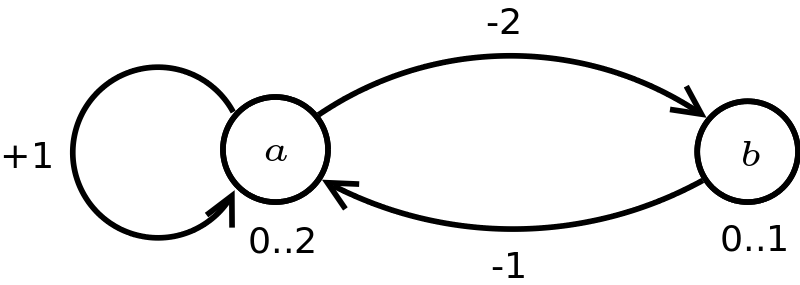
\includegraphics[width=7cm]{figs/gi-sans-multiplexe}
  \caption{Un exemple de graphe d'interaction simple \cite{richard-comet-bernot-08} : les n\oe uds modélisent les gènes et les arcs leurs influences mutuelles. Ici, le gène $a$ s'auto-active tandis que les deux gènes $a$ et $b$ s'inhibent mutuellement. Les valeurs sous les n\oe uds indiquent les niveaux d'expressions accessibles pour chaque gène.}
  \label{rrg-gi-sans-multiplexe}
\end{figure}

Dans le modèle originellement proposé par Thomas, un gène pouvant potentiellement exercer une influence sur un autre gène est relié à celui-ci par un arc (dirigé vers ce dernier) étiqueté par une valeur de seuil et un type d'influence (qui consiste en une information booléenne car l'influence ne peut être que positive ou négative). Ainsi, pour savoir si ce gène exerce son influence sur le second gène à un instant donné, il suffit de comparer le niveau d'expression de ce gène à cette valeur de seuil, à l'aide d'une simple relation d'inégalité : une interaction positive (resp. négative) ne pourra avoir lieu que si le niveau d'expression du gène est supérieur (resp. inférieur) au seuil. Les assertions qui conditionnent les influences entre gènes consistent donc uniquement en des inégalités.

Si ce modèle permet de représenter une grande partie des relations d'influences des systèmes étudiés, il subsiste cependant des cas pour lesquels il échoue à représenter certains comportements. On peut notamment citer le cas où plusieurs gènes doivent s'associer pour exercer une influence ; ce cas ne peut pas être représenté car les arcs d'un graphe d'interaction ne peuvent partir que d'un unique n\oe ud, pour n'arriver que dans un unique n\oe ud. De même, on pourrait imaginer une situation où un gène peut exercer une influence sur un autre lorsque son niveau d'expression \og n'est pas trop élevé \fg, et qu'il se trouve donc dans un intervalle ; à nouveau, les inégalités simples ne permettent pas de prendre ce type de comportement en compte.

Afin de combler cette lacune, la notion de \emph{multiplexe} a été proposée pour de permettre la modélisation de comportements plus complexes \cite{bernot-comet-khalis-08, khalis-bernot-comet-richard-roux-siebert-UnPublished}. Les multiplexes viennent s'ajouter aux étiquettes des arcs du modèle présenté précédemment. Ils se présentent comme des n\oe uds d'un type différent de ceux représentant les gènes au sein du graphe d'interactions, et comportent :
\begin{itemize}
  \item un nom,
  \item une assertion, appelée \emph{condition d'influence}, exprimée en logique modale et qui dépend uniquement de ses prédécesseurs dans le graphe (gènes ou autres multiplexes).
\end{itemize}
Ainsi, un gène pouvant potentiellement exercer une influence sur un autre possède un arc sortant qui pointe vers un multiplexe, et ce multiplexe possède à son tour un arc sortant pointant vers le gène final. L'influence aura effectivement lieu si la condition d'influence du multiplexe est satisfaite. Dans ce modèle, on permet qu'un multiplexe possède un arc sortant vers un autre multiplexe, à condition qu'il n'existe pas de cycle ne faisant intervenir que des multiplexes. La figure~\ref{rrg-gi-avec-multiplexe} reprend l'exemple précédent en le complétant avec les multiplexes correspondants.

\begin{figure}[ht]
  \centering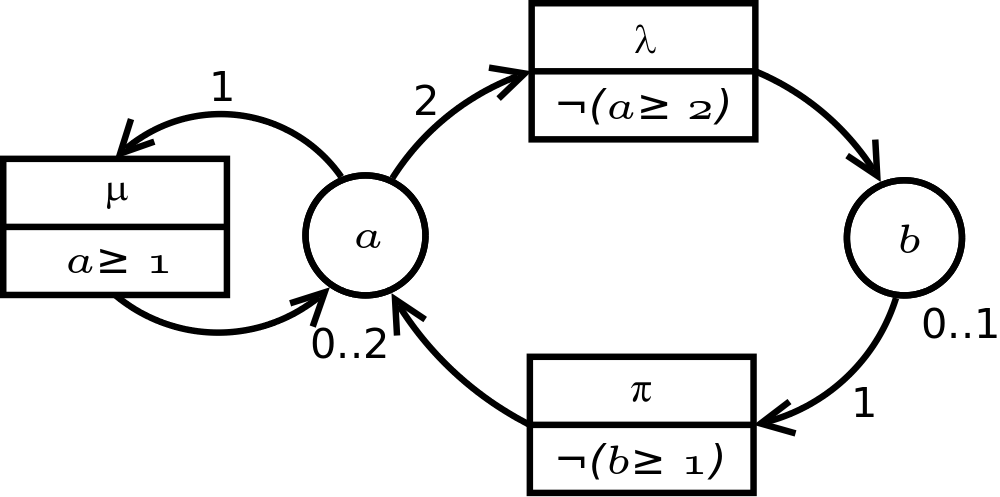
\includegraphics[width=7cm]{figs/gi-avec-multiplexe}
  \caption{Un exemple de graphe d'interaction avec multiplexes : les conditions d'influence sont précisées dans un nouveau type de n\oe ud appelé multiplexe. Pour comparaison, ce graphe définit exactement le même système de gènes que celui de la figure~\ref{rrg-gi-sans-multiplexe}.}
  \label{rrg-gi-avec-multiplexe}
\end{figure}

\section{Graphe d'interaction et paramétrisation}
Définissons le modèle du graphe d'interaction de façon formelle, d'après la description de la partie précédente. Il est à noter que les n\oe uds du graphe d'interaction représentant les gènes sont appelés \emph{variables}. Dans la suite, on utilisera les deux dénominations, bien que le terme de \emph{gène} semble plus adapté à une description biologique des phénomènes mis en jeu.
\begin{definition}[Graphe d'interaction]
Un \emph{graphe d'interaction avec multiplexes} est un quadruplet $G = (V ; M ; E_V ; E_M)$ qui vérifie les propriétés suivantes :
\begin{itemize}
  \item $(V \cup M ; E_V \cup E_M)$ est un graphe orienté et étiqueté, dont les n\oe uds sont $V \cup M$ et les arcs sont $E_V \cup E_M$, vérifiant les contraintes suivantes :
  \begin{itemize}
    \item les ensembles $V$ et $M$ sont finis et disjoints ; les éléments de $V$ sont appelés \emph{variables} et ceux de $M$ sont appelés \emph{multiplexes},
    \item les arcs de $E_V$ ont pour source une variable et pour cible un multiplexe, tandis que les arcs de $E_M$ ont pour source un multiplexe et pour cible une variable ou un autre multiplexe,
    \item tout cycle de $G$ contient au moins une variable,
  \end{itemize}
  \item toute variable $v$ de $V$ est étiquetée par un entier positif $b_v$ qui est appelé son \emph{plafond},
  \item tout arc de $E_V$ est étiqueté par un entier positif $s$ inférieur ou égal au plafond de sa variable source et appelé \emph{seuil} ; on note un tel arc $v \xrightarrow{s} m$ où $v$ est sa variable source et $m$ est son multiplexe cible.
  \item tout multiplexe $m$ de $M$ est étiqueté par une formule $\varphi_m$ appartenant au langage $\mathcal{L}_m$ défini inductivement par :
  \begin{itemize}
    \item si $v \xrightarrow{s} m$ appartient à $E_V$ alors $v \geq s$ est un atome de $\mathcal{L}_m$,
    \item si $m' \xrightarrow{} m$ appartient à $E_M$ alors $m'$ est un atome de $\mathcal{L}_m$,
    \item si $\varphi$ et $\psi$ appartiennent à $\mathcal{L}_m$ alors $\neg \varphi$, $\varphi \wedge \psi$ et $\varphi \vee \psi$ sont des atomes de $\mathcal{L}_m$.
  \end{itemize}
\end{itemize}
\end{definition}
On retrouve dans cette définition tous les éléments développés en introduction. Il est à noter que l'introduction de multiplexes ne supprime pas totalement les étiquettes déjà présentes sur les arcs partant des variables. En effet, si l'information concernant le type d'influence (activation ou inhibition) est ici portée par l'assertion du multiplexe, il est en revanche toujours nécessaire de connaître le seuil au delà duquel le niveau d'expression du gène jouera un rôle dans cette assertion.

Afin de pouvoir étudier le comportement d'un système modélisé grâce à l'outil développé ici, il est nécessaire d'introduire une certaine forme de dynamique. Cette notion était déjà présente durant toute la partie d'introduction, lorsqu'il était question des niveaux d'expression des différents gènes (mesurés à partir de la quantité de protéine produite et présente dans le milieu). L'état d'un graphe d'interaction se définit alors aisément comme l'ensemble des niveaux d'expression des variables qui le composent.
\begin{definition}[État d'un graphe d'interaction]
Un \emph{état} d'un graphe d'interaction $G = (V ; M ; E_V ; E_M)$ est une fonction $\eta : V \rightarrow \mathbb{N}$ telle que pour toute variable $v$ de $V$, on ait : $\eta(v) \leq b_v$. $\eta(v)$ est appelé le \emph{niveau d'expression} de $v$.
\end{definition}

Il est important de noter que si l'état d'un graphe d'interaction représente l'état des gènes qui le composent à un instant donné, la notion de temps n'intervient cependant à aucun moment dans le modèle. En effet, la dynamique du graphe d'interactions est vue comme une succession d'instants, mais il n'est en aucun cas question de quantifier la durée qui sépare deux de ces instants. On fera d'ailleurs dans la partie suivante l'hypothèse selon laquelle une durée suffisamment longue s'écoule entre deux changements d'état successifs du graphe.

Pour terminer cette première partie concernant les graphes d'interaction, il nous faut formaliser les possibilités d'influence entre les variables au travers des multiplexes. Dans un état donné, un gène reçoit une influence d'un certain nombre d'autres gènes \textit{via} certains multiplexes. Plus précisément, ces multiplexes doivent posséder un arc sortant vers le gène en question, et leur assertion doit être satisfaite. On parvient donc à la définition suivante, où la notation $G^{-1}(x)$ représente l'ensemble des prédécesseurs d'un n\oe ud $x$ du graphe.
\begin{definition}[Ressources d'une variable]
Étant donnés un graphe d'interaction $G = (V ; M ; E_V ; E_M)$ et un état $\eta$ de $G$, l'ensemble des \emph{ressources} d'une variable $v$ de $V$ pour l'état $\eta$, qu'on note $\rho(v, \eta)$, est l'ensemble des multiplexes $m$ de $G^{-1}(v)$ tels que $\varphi_m$ est satisfaite. L'interprétation de la formule $\varphi_m$ d'un multiplexe $m$ est inductivement définie par :
\begin{itemize}
  \item si $\varphi_m$ est réduite à un atome $v \geq s$, où $v \in G^{-1}(m)$ et $(v \xrightarrow{s} m) \in E_V$, alors $\varphi_m$ est satisfaite ssi $\eta(v) \geq s$,
  \item si $\varphi_m$ est réduite à un atome $m' \in M$, où $m' \in G^{-1}(m)$, alors $\varphi_m$ est satisfaite ssi $\varphi_{m'}$,
  \item si $\varphi_m$ est une formule constituée d'atomes et de connecteurs logiques, alors :
  \begin{itemize}
    \item $\varphi_m \equiv \neg \psi$ est satisfaite ssi $\psi$ n'est pas satisfaite,
    \item $\varphi_m \equiv \psi_1 \wedge \psi_2$ est satisfaite ssi $\psi_1$ et $\psi_2$ sont satisfaites,
    \item $\varphi_m \equiv \psi_1 \vee \psi_2$ est satisfaite ssi $\psi_1$ est satisfaite ou $\psi_2$ est satisfaite.
  \end{itemize}
\end{itemize}
\end{definition}
Le symbole $\equiv$ utilisé dans cette définition et dans les définitions à venir indique l'équivalence entre deux assertions.

\section{Réseau de régulation et graphe d'états asynchrone}
\label{rrg-reseau-de-regulation}
Si la notion d'interaction a largement été abordée jusqu'ici, il n'a pas encore été question de quantifier cette interaction. En effet, si on peut modéliser le fait qu'un gène possède une influence sur un autre gène, car faisant partie de ses ressources, et pouvant donc contraindre ce dernier à changer de niveau d'expression, le modèle actuel ne contient pas d'information quant au niveau vers lequel le gène influencé sera attiré. Il reste donc à définir une \og carte \fg{} des interactions spécifiant, selon les ressources d'une variable, l'état vers lequel celle-ci sera attirée.
\begin{definition}[Réseau de régulation]
Un \emph{réseau de régulation génétique avec multiplexes} est un couple $(G ; \mathcal{K})$ où :
\begin{itemize}
  \item $G = (V ; M ; E_V ; E_M)$ est un graphe d'interaction,
  \item $\mathcal{K} = \{k_{v, \omega}\}$ est une famille de paramètres indexés par $v \in V$ et $\omega \subset G^{-1}(v)$ telle que chaque $k_{v, \omega}$ de $\mathcal{K}$ soit un entier vérifiant : $0 \leq k_{v, \omega} \leq b_v$.
\end{itemize}
$\mathcal{K}$ est appelée \emph{paramétrisation} de $G$ (ou de $N$).
\end{definition}

Le réseau de régulation, extension du graphe d'interaction, est un outil complet comprenant toutes les informations concernant le système étudié et sa dynamique. Il est important de noter qu'il n'existe pas une unique paramétrisation pour un graphe d'interaction donné. En général, le nombre de paramétrisations possibles est très important et constitue l'une des limitations de ce modèle \cite{richard-comet-bernot-08}. Cependant, nous ne nous intéresserons pas dans ce chapitre à leur recherche et travaillerons avec des paramétrisations données. La figure~\ref{rrg-ex-parametrisation} donne un exemple de paramétrisation pour le graphe donné en exemple plus haut.\\

\begin{figure}[htbp]
  %\begin{center}
  \centering%\begin{tabular}{ccc}
  %\leavevmode
  %\subfloat[Graphe d'interaction]{
    \begin{tabular}{c}
      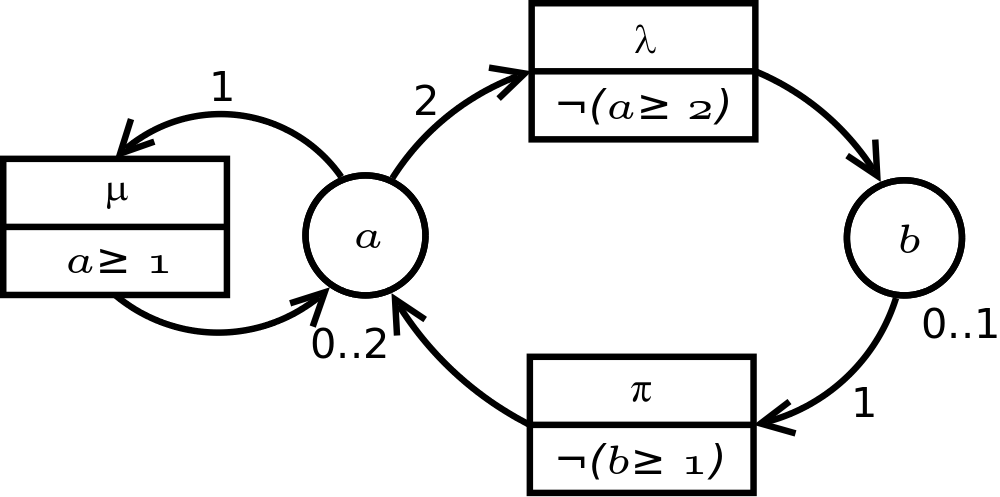
\includegraphics[width=7cm]{figs/gi-avec-multiplexe}
      \\\small(a)
    \end{tabular}
%}
\hspace{.5cm} %&%&
    \begin{tabular}{c}
  %\subfloat[Paramétrisation]{
  %\begin{tabular}[b]{cc}
    $\begin{array}{c|c}
      \omega & k_{a, \omega}\\
      \hline
      \emptyset & 2\\
      \{\mu\} & 2\\
      \{\pi\} & 0\\
      \{\mu, \pi\} & 0
    \end{array}$\hspace{.5cm}%&
    $\begin{array}{c|c}
      \omega & k_{b, \omega}\\
      \hline
      \emptyset & 1\\
      \{\lambda\} & 0
    \end{array}$%\end{tabular}%}
    \\\small(b)
    \end{tabular}
%}  %\end{tabular}
%  \subfloat[test]{
%    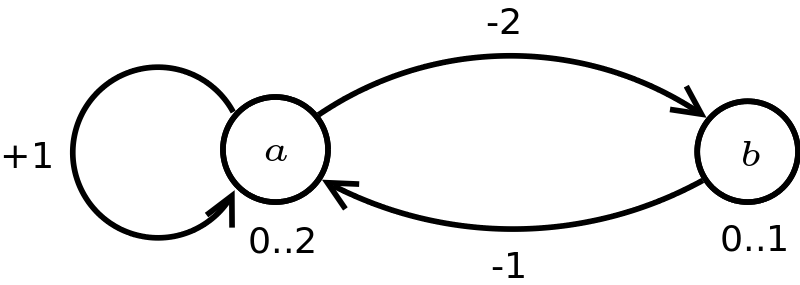
\includegraphics[width=7cm]{figs/gi-sans-multiplexe}} %&
  %\end{center}
  \caption{Un exemple réseau de régulation génétique comprenant un graphe d'interaction (a) et une paramétrisation (b). \cite{richard-comet-bernot-08}}
  \label{rrg-ex-parametrisation}
\end{figure}

Afin de pouvoir étudier les différents scénarios possibles, il faut énumérer les états accessibles par le réseau de régulation (pour un graphe d'interaction et une paramétrisation associée donnés). Cela s'effectue aisément en calculant le graphe d'états du réseau de régulation. Cependant, la notion de successeur d'un état ne saurait se satisfaire d'une définition trop générale. En effet, le modèle étudié ici observe le système en des instants successifs sans aucune quantification temporelle ; or il est nécessaire de prendre en compte la vitesse des évolutions les unes par rapport aux autres afin de limiter les comportements. L'observation montre que l'évolution d'un gène depuis un niveau d'expression jusqu'à un autre est un processus suffisamment lent (du fait de sa complexité biologique) pour ne pas pouvoir être considéré comme instantané, et que ce temps varie beaucoup entre les gènes \cite{richard-comet-bernot-08}. Il est donc possible d'approximer le comportement du système à l'aide d'une approche asynchrone : un seul gène à la fois est en mesure d'évoluer entre deux états successifs du système. Cette évolution ne peut constituer qu'en un changement de niveau d'expression d'une unité vers le haut ou vers le bas. Ainsi, l'observation de l'évolution du système est ramenée à l'observation d'une série d'instants situés entre deux changements d'état successifs.

Nous pouvons alors définir formellement un changement d'état. Nous allons cependant au préalable définir un outil supplémentaire qui permet de généraliser la notion de changement de niveau d'expression en précisant la direction vers laquelle est attiré un gène (\textit{i.e.} vers un niveau d'expression supérieur ou inférieur).
\begin{definition}[Fonction de direction]
Pour un réseau de régulation $N = (G ; \mathcal{K})$ et un état $\eta$ de $G = (V ; M ; E_V ; E_M)$ donnés, la \emph{fonction de direction} $d : V \rightarrow \{-1 ; 0 ; 1\}$ est définie par :
$$\forall v \in V, d(v) = 
\left\{\begin{array}{r l}
-1 & \text{si}\ \eta(v) > k_{v, \rho(v, \eta)}\\
0 & \text{si}\ \eta(v) = k_{v, \rho(v, \eta)}\\
+1 & \text{si}\ \eta(v) < k_{v, \rho(v, \eta)}
\end{array}\right.$$
\end{definition}

Comme nous l'avons évoqué, un successeur possible d'un état est un autre état identique au premier, excepté pour un gène qui a vu son niveau d'expression augmenté ou diminué d'une unité.
\begin{definition}[Successeur d'un état]
Si $N = (G ; \mathcal{K})$ est un réseau de régulation et $\eta$ un état de $G$ donnés, un état $\eta'$ de $G$ est un \emph{successeur} de $\eta$ ssi :
\begin{itemize}
  \item il existe une variable $u$ telle que $\eta'(u) = \eta(u) + d(u)$ et $d(u) \neq 0$,
  \item pour toute autre variable  $v \neq u$, on a : $\eta'(u) = \eta(u)$.
\end{itemize}
\end{definition}

On peut alors calculer un graphe des états à l'aide de la définition précédente de successeur d'un état.
\begin{definition}[Graphe d'états asynchrone]
Étant donné un réseau de régulation génétique $N = (G ; \mathcal{K})$, on appelle \emph{graphe d'états asynchrone} le graphe $\mathcal{S}_N$ vérifiant les propriétés suivantes :
\begin{itemize}
  \item l'ensemble des n\oe uds de $\mathcal{S}_N$ est l'ensemble des états possibles de $G$ (isomorphe au produit cartésien $\prod_{v \in V} [0 ; b_v]$),
  \item l'ensemble des arcs de $\mathcal{S}_N$ est l'ensemble des couples $(\eta ; \eta')$ tels que $\eta'$ est un successeur de $\eta$.
\end{itemize}
\end{definition}

Le système de transitions fini obtenu par cette définition ne possède pas explicitement d'état initial car on considère que tout état peut potentiellement en être un (selon l'instant où l'observation débute).

À titre d'exemple, la figure~\ref{rrg-graphe-d-etats} donne le graphe d'états associé à l'exemple donné précédemment.

\begin{figure}[ht]
  \centering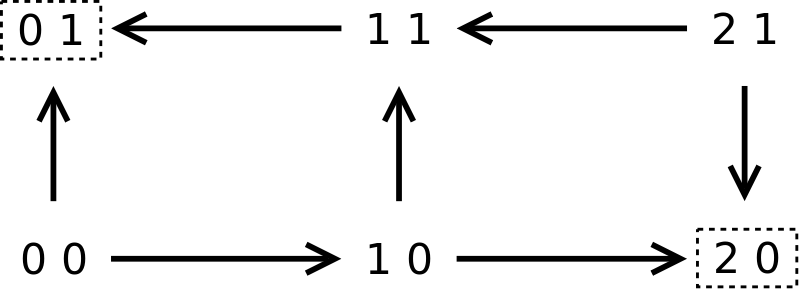
\includegraphics[width=7cm]{figs/graphe-d-etats}
  \caption{Le graphe d'états obtenu à partir du réseau de régulation de la figure~\ref{rrg-ex-parametrisation} \cite{richard-comet-bernot-08}. Chaque état est un couple du niveau d'expression des gènes $a$ et $b$, dans cet ordre.}
  \label{rrg-graphe-d-etats}
\end{figure}

Les graphes d'états offrent un outil efficace pour l'étude des réseaux de régulation. Cependant, il est important de noter à ce stade que la génération d'un graphe d'états est soumise à l'explosion combinatoire du nombre de ses états. En effet, l'ajout d'une variable dans le graphe d'interaction aura pour double conséquence :
\begin{itemize}
  \item d'ajouter un niveau d'expression à prendre en compte,
  \item de potentiellement faire augmenter le plafond d'une partie des autres gènes déjà présents dans le graphe d'interaction.
\end{itemize}
Ces deux éléments ont pour conséquence directe l'augmentation de la taille de graphe d'états, et peuvent entraîner des problèmes de mémoire et de temp d'exécution.

\section{Quelques définitions supplémentaires}
Certaines structures fréquemment rencontrées au sein des graphes d'états asynchrones obtenus par cette méthode sont décrites dans \cite{richard-comet-bernot-08}. Elles seront définies et expliquées dans la suite, et quelques théorèmes les concernant seront aussi donnés. Dans toute cette partie, on considère un réseau de régulation $N = (G ; \mathcal{K})$ dont $G$ est le graphe d'interaction et $\mathcal{K}$ la paramétrisation, et on appelle $\mathcal{S}_N$ son graphe d'états asynchrone.

\begin{definition}[Domaine piège]
Un \emph{domaine piège} de $\mathcal{S}_N$ est un sous-ensemble $T$ des n\oe uds du graphe tel que pour toute transition $x \rightarrow y$ dans $\mathcal{S}_N$, si $x \in T$, alors $y \in T$.
\end{definition}
D'après cette définition, un domaine piège est donc un sous-ensemble de configurations du système dont on ne peut sortir. Tout graphe d'états contient au moins un cas particulier de domaine piège, qui est l'ensemble de tous ses états.

\begin{definition}[Attracteur]
Un \emph{attracteur} de $\mathcal{S}_N$ est un domaine piège qui ne contient pas d'autre domaine piège que lui-même.
\end{definition}
La notion d'attracteur restreint celle de domaine piège en le caractérisant de plus petit domaine piège du point de vue de la relation d'inclusion. On peut donner quelques propriétés intéressantes concernant les attracteurs.

\begin{propriete}[Propriétés sur les attracteurs]~
\begin{itemize}
  \item Les attracteurs sont en fait les composantes fortement connexes du graphe (car si deux éléments $x$ et $y$ appartiennent au même attracteur, alors il existe un chemin de $x$ à $y$ et un chemin de $y$ à $x$).
  \item Tout graphe d'états contient au moins un attracteur (car il contient au moins un domaine piège).
  \item Les attracteurs sont mutuellement disjoints.
  \item Depuis tout état du graphe, il existe au moins un chemin conduisant à un attracteur.
\end{itemize}
\end{propriete}

\begin{definition}[État stable]
Un état puits (\textit{i.e.} qui ne possède aucun arc sortant) de $\mathcal{S}_N$ est appelé \emph{état stable}.
\end{definition}

Un état stable est un cas particulier d'attracteur (et donc de domaine piège) qui contient un seul élément. Lorsqu'un état stable est atteint, le système n'est plus en mesure d'évoluer. Les états stables d'un réseau de régulation peuvent être la conséquence de la \og victoire \fg{} de l'expression d'un ensemble de gènes sur un autre, ce dernier ne pouvant plus prendre le dessus. La figure~\ref{rrg-graphe-d-etats} contient deux attracteurs, entourés en pointillés ; ils modélisent le fait que l'un ou l'autre des deux gènes a gagné un niveau d'expression suffisant pour ne plus subir l'influence de l'autre gène.

Un attracteur composé de plus d'un seul élément (par opposition à un état stable) est appelé qualifié de \emph{cyclique}. Cette dénomination traduit le fait qu'un attracteur qui n'est pas un état stable contient nécessairement un cycle. Ce type d'attracteur peut potentiellement modéliser tout type de comportement oscillant d'un système.


\chapter{Logiques temporelles}
\label{tempo}
Le modèle de Thomas permet d'obtenir un graphe d'états asynchrone (cf. section~\ref{rrg-reseau-de-regulation}) à partir d'un graphe d'interaction et d'une paramétrisation associée. Historiquement, les graphes sont étudiés à l'aide des logiques temporelles car celles-ci proposent un moyen commode \mbox{d'exprimer} des assertions sur des chemins. Ce chapitre sera l'occasion de présenter la logique CTL*, et de voir en quoi elle peut être utile à l'étude des réseaux de régulation génétiques.

\section{Introduction}
Les logiques temporelles ont été proposées afin de permettre de décrire des propriétés sur les chemins des graphes. L'idée à l'origine de la formulation de ce type de logiques est naturellement l'étude des systèmes modélisés par des graphes. Plusieurs logiques ayant des pouvoirs d'expression différents ont été proposées, et nous n'étudierons ici que la logique CTL*, qui permet d'exprimer des propriétés sur les états d'un graphe (contrairement à la logique de Hennessy-Milner par exemple, qui exprime des propriétés sur les transitions) selon un temps logique (constitué d'une succession discrète d'états et non d'un écoulement continu du temps) \cite{arnold-92, berard-08}. Cette logique s'applique à l'ensemble des structures de Kripke, qui est la famille de graphes orientés dont les états sont étiquetés par des propositions atomiques ; dans la suite de ce chapitre on pourra confondre les notions de graphe et de structure de Kripke. La logique CTL* étant elle-même composée des logiques temporelles CTL et LTL, ces deux dernières seront tout d'abord définies dans les sections suivantes.

\subsection*{Définitions préalables}
Les logiques LTL et CTL s'appliquent à des structures de Kripke, qui représentent un type de graphe particulier.
\begin{definition}[Structure de Kripke]
Une \emph{structure de Kripke} sur un ensemble $\mathsf{Prop}$ est un couple $\mathcal{S} = (Q, l)$ où :
\begin{itemize}
  \item $Q$ est un graphe ;
  \item $l : Q \mapsto \mathcal{P}(\mathsf{Prop})$ est la fonction d'étiquetage.
\end{itemize}
De plus, si une propriété $P \in \mathsf{Prop}$ et un état $q$ de $Q$ vérifient $P \in l(q)$, on dit alors que $P$ est vraie dans $q$.
\end{definition}

Il est de plus nécessaire de préciser la notion de chemin maximal, qui étend celle de chemin infini, souvent rencontrée en théorie des graphes.
\begin{definition}[Chemin maximal]
Un \emph{chemin maximal} sur un graphe est un chemin qui est soit infini, soit dont le dernier état est un état puits (\textit{i.e.} qui n'est l'origine d'aucune transition).
\end{definition}
Dans la suite, si $\sigma$ est un chemin sur un graphe donné, on note $\sigma_i$ son $i^\text{ème}$ état, le premier état ayant l'indice zéro.

\section{La logique LTL}
Soit une structure de Kripke $\mathcal{S}$ donnée. La logique temporelle linéaire, abrégée en LTL pour \textit{linear temporal logic} (on trouve parfois aussi PLTL), s'interprète sur la première position d'un chemin maximal $\sigma : q_0 \rightarrow q_1 \rightarrow q_2 \ldots$ du graphe. Elle se formule à l'aide de la grammaire suivante :
  $$\varphi, \psi ::= \texttt{vrai} \mid P \mid \neg \varphi \mid \varphi \wedge \psi \mid \textsf{X} \varphi \mid \varphi \textsf{U} \psi$$
où $P$ est une proposition atomique. La sémantique de la logique LTL est ensuite définie inductivement par :\\
\begin{tabular}{ll}
  $\sigma \models \texttt{vrai}$ & quel que soit $\sigma$,\\
  $\sigma \models P$ & ssi $P$ est vraie dans $\sigma_0$,\\
  $\sigma \models \neg \varphi$ & ssi $\sigma_0$ ne satisfait pas $\varphi$,\\
  $\sigma \models \varphi \wedge \psi$ & ssi $\sigma_0$ vérifie $\varphi$ et $\psi$,\\
  $\sigma \models \mathsf{X} \varphi$ & ssi $\sigma = \sigma_0.\sigma'$ et $\sigma' \models \varphi$,\\
  $\sigma \models \varphi \mathsf{U} \psi$ & ssi il existe $i \in \mathbb{N}$ tel que $\sigma_i \models \psi$ et pour tout $k \in \mathbb{N}, 0 \leq k \leq i, \sigma_k \models \varphi$.
\end{tabular}\\

La modalité $\mathsf{X}$ (pour \emph{neXt}) permet de vérifier une propriété sur l'état suivant sur le chemin étudié : en effet, $\mathsf{X} \varphi$ est satisfaite dans un état lorsque $\varphi$ est satisfaite dans l'état suivant. La modalité $\mathsf{U}$ (pour \emph{Until}) permet de vérifier qu'une propriété est vraie jusqu'à ce qu'un autre le soit : ainsi, $\varphi \mathsf{U} \psi$ est satisfaite dans un état s'il existe un état dans le futur où $\psi$ est satisfaite, et si $\varphi$ est tout le temps satisfaite sur le chemin avant cela. Les modalités $\neg$ et $\wedge$ sont directement tirées de la logique modale ; on peut les utiliser pour définir des opérateurs modaux supplémentaires (tels que $\vee$ ou $\Rightarrow$). Enfin, on peut aussi définir les opérateurs temporels suivants :
\begin{itemize}
  \item $\mathsf{F} \varphi \equiv \texttt{vrai} \mathsf{U} \varphi$, signifie que la propriété $\varphi$ sera satisfaite un jour (\textit{Fatalement}),
  \item $\mathsf{G} \varphi \equiv \neg \mathsf{F} (\neg \varphi)$, signifie que la propriété $\varphi$ est toujours vérifiée (\textit{Globalement}).
\end{itemize}
On trouve parfois aussi dans la littérature les symboles $\Diamond$ à la place de $\mathsf{F}$ et $\Box$ à la place de $\mathsf{G}$.\\

Afin d'illustrer le fonctionnement de cette logique à l'aide d'un exemple, considérons un graphe dont les états sont étiquetés par le langage $\mathcal{L} = \{a, b\}$. On déduit de ce graphe une structure de Kripke en paramétrant chaque état par une propriété $P_x$ où $x \in \mathcal{L}$, de façon à ce que $P_x$ soit vraie dans un état si et seulement si cet état est étiqueté par $x$. On souhaite caractériser par la logique LTL tous les chemins qui appartiennent aux mots infinis : $(a^*.a.b)^{\omega}$, \textit{i.e.} les mots qui commencent par $a$, et contiennent au plus une occurrence successive de $b$.

Le fait qu'un état étiqueté par $b$ soit toujours suivi d'un état étiqueté par $a$ se traduit par la formule :
\begin{listesanspuce}
  \item $P_b \Rightarrow \mathsf{N}P_a$
\end{listesanspuce}
Afin de généraliser cette formule à tous les états d'un chemin, il suffit d'utiliser l'opérateur de globalité :
\begin{listesanspuce}
  \item $\mathsf{G}(P_b \Rightarrow \mathsf{N}P_a)$
\end{listesanspuce}
Les chemins qui forment les mots $(a^*.a.b)^{\omega}$ sont donc ceux qui vérifient cette formule.

\section{La logique CTL}
Soit une structure de Kripke $\mathcal{S}$ donnée. La logique temporelle arborescente, abrégée en CTL pour \textit{computation tree logic}, s'interprète sur un état $q$ du graphe. On notera dans la suite $\mathcal{E}^\mathcal{S}_q$ l'arbre des chemins maximaux de $\mathcal{S}$ partant de $q$. Elle se formule à l'aide de la grammaire suivante :
  $$\varphi, \psi ::= \texttt{vrai} \mid P \mid \neg \varphi \mid \varphi \wedge \psi \mid \textsf{EX} \varphi \mid \textsf{AX} \varphi \mid \varphi \textsf{EU} \psi \mid \varphi \textsf{AU} \psi$$
où $P$ est une proposition atomique. La sémantique de la logique CTL est alors définie inductivement par :\\
\begin{tabular}{ll}%p{13cm}}
  $q \models \texttt{vrai}$ & quel que soit $q$,\\
  $q \models P$ & ssi $P$ est vraie dans $q$,\\
  $q \models \neg \varphi$ & ssi $q$ ne satisfait pas $\varphi$,\\
  $q \models \varphi \wedge \psi$ & ssi $q$ vérifie $\varphi$ et $\psi$,\\
  $q \models \mathsf{EX} \varphi$ & ssi il existe un chemin maximal $\sigma$ de $\mathcal{E}^\mathcal{S}_q$ tel que $\sigma_1 \models \varphi$,\\
  $q \models \mathsf{AX} \varphi$ & ssi tous les chemins maximaux $\sigma$ de $\mathcal{E}^\mathcal{S}_q$ vérifient $\sigma_1 \models \varphi$,\\
  $q \models \varphi \mathsf{EU} \psi$ & ssi il existe un chemin maximal $\sigma$ de $\mathcal{E}^\mathcal{S}_q$ et un entier $i \in \mathbb{N}$ tels que $\sigma_i \models \psi$\\&\quad et pour tout $k \in \mathbb{N}, 0 \leq k \leq i, \sigma_k \models \varphi$.\\
  $\sigma \models \varphi \mathsf{AU} \psi$ & ssi pour tout chemin maximal $\sigma$ de $\mathcal{E}^\mathcal{S}_q$, il existe un entier $i \in \mathbb{N}$ tel que $\sigma_i \models \psi$\\&\quad et pour tout $k \in \mathbb{N}, 0 \leq k \leq i, \sigma_k \models \varphi$.
\end{tabular}\\

Les quantificateurs $\mathsf{E}$ et $\mathsf{A}$ sont respectivement les quantificateurs existentiel et universel sur les chemins maximaux de l'arbre d'exécution. Ils ont donc des rôles qui s'apparient aux quantificateurs $\exists$ et $\forall$ de la logique du premier ordre. Les modalités $\mathsf{EX}$ et $\mathsf{AX}$ (resp. $\mathsf{EU}$ et $\mathsf{AU}$) sont donc semblables à une modalité $\mathsf{X}$ de la logique LTL (resp. $\mathsf{U}$) couplée à un quantificateur sur les chemins sortants de l'état considéré. Cependant, malgré ces similitudes, les deux logiques n'expriment strictement pas les mêmes comportements \cite{berard-08}.

A partir des opérateurs précédents, on peut aussi définir les abréviations suivantes :
\begin{itemize}
  \item $\mathsf{EF} \varphi \equiv \mathsf{E} \texttt{vrai} \mathsf{U} \varphi$, signifie qu'il existe un chemin maximal sur lequel la propriété $\varphi$ sera satisfaite un jour ($\varphi$ est dite accessible),
  \item $\mathsf{AF} \varphi \equiv \mathsf{A} \texttt{vrai} \mathsf{U} \varphi$, signifie que pour tous les chemins maximaux, la propriété $\varphi$ sera satisfaite un jour ($\varphi$ est dite inévitable),
  \item $\mathsf{EG} \varphi \equiv \neg \mathsf{AF} (\neg \varphi)$, signifie qu'il existe un chemin maximal où la propriété $\varphi$ sera toujours satisfaite ($\varphi$ est dite préservable),
  \item $\mathsf{AG} \varphi \equiv \neg \mathsf{EF} (\neg \varphi)$, signifie que $\varphi$ sera toujours satisfaite pour tous les chemins maximaux.
\end{itemize}~

La logique CTL peut entre autres être utilisée pour formuler des propriétés de sûreté. Par exemple, supposons que la structure de Kripke $\mathcal{S}$ modélise un système pouvant rencontrer des erreurs, les états potentiellement défaillants (\textit{i.e.} pouvant provoquer une erreur) étant paramétrés par $P$. On souhaite s'assurer que de telles erreurs peuvent être prises en charge par un module de secours, qui est lancé dans les états paramétrés par $Q$. Ainsi, dès qu'un état vérifiant $P$ est rencontré, il faut qu'un état vérifiant $Q$ puisse être rencontré par la suite. Cela se traduit par :
\begin{listesanspuce}
  \item $P \Rightarrow \mathsf{EF}Q$
\end{listesanspuce}
Cette propriété doit être vérifiée pour toutes les exécutions possibles, soit :
\begin{listesanspuce}
  \item $\mathsf{AG}(P \Rightarrow \mathsf{EF})$
\end{listesanspuce}

Si on a défini un état initial dans notre structure de Kripke, il faut que cet état vérifie cette formule. Si on se permet de débuter une exécution à partir de n'importe quel état, alors tous les états de la structure de Kripke doivent la vérifier.

\section{La logique CTL*}
La logique CTL* se définit de façon intuitive comme la \og réunion \fg{} des deux logiques présentées précédemment. Elle s'exprime donc en fonction de modalités portant sur les états (comme CTL) et sur les chemins (comme LTL).

De façon formelle, CTL* est l'ensemble des formules d'état $\varphi_s$ définies à l'aide de la grammaire :
  $$\varphi_s, \psi_s ::= \texttt{vrai} \mid P \mid \neg \varphi_s \mid \varphi_s \wedge \psi_s \mid \textsf{E} \varphi_p \mid \textsf{A} \varphi_p$$
où $P$ est une proposition atomique, et où on définit les formules de chemins $\varphi_p$ à l'aide de la grammaire :
  $$\varphi_p, \psi_p ::= \texttt{vrai} \mid \varphi_s \mid \varphi_p \wedge \psi_p \mid \textsf{X} \varphi_p \mid \varphi_p \textsf{U} \psi_p$$
La sémantique des formules d'états est définie inductivement par :\\
\begin{tabular}{ll}%p{13cm}}
  $q \models \texttt{vrai}$ & quel que soit $q$,\\
  $q \models P$ & ssi $P$ est vraie dans $q$,\\
  $q \models \neg \varphi_s$ & ssi $q$ ne satisfait pas $\varphi_s$,\\
  $q \models \varphi_s \wedge \psi_s$ & ssi $q$ vérifie $\varphi_s$ et $\psi_s$,\\
  $q \models \mathsf{E} \varphi_p$ & ssi il existe un chemin maximal $\sigma$ de $\mathcal{E}^\mathcal{S}_q$ tel que $\sigma \models \varphi_p$,\\
  $q \models \mathsf{A} \varphi_p$ & ssi tous les chemins maximaux $\sigma$ de $\mathcal{E}^\mathcal{S}_q$ vérifient $\sigma \models \varphi_p$.\\
\end{tabular}\\
La sémantique des formules de chemins est définie inductivement par :\\
\begin{tabular}{ll}%p{13cm}}
  $\sigma \models \texttt{vrai}$ & quel que soit $\sigma$,\\
  $\sigma \models \varphi_s$ & ssi $\sigma_0 \models \varphi_s$,\\
  $\sigma \models \varphi_p \wedge \psi_p$ & ssi $\sigma$ vérifie $\varphi_p$ et $\psi_p$,\\
  $\sigma \models \mathsf{X} \varphi_p$ & ssi $\sigma = \sigma_0.\sigma'$ et $\sigma' \models \varphi_p$,\\
  $\sigma \models \varphi_p \mathsf{U} \psi_p$ & ssi il existe $i \in \mathbb{N}$ tel que $\sigma_i \models \psi_p$ et pour tout $k \in \mathbb{N}, 0 \leq k \leq i, \sigma_k \models \varphi_p$.
\end{tabular}\\

\section{Cas d'utilisation et discussion}
La logique modale se prête bien à l'étude d'entités non dynamiques en les caractérisant grâce à des propriétés atomiques ou composées de propriétés atomiques. Cependant, l'étude d'une entité dynamique (capable d'évoluer dans le temps) n'est pas possible à l'aide de la logique modale seule, car celle-ci ne possède pas de pouvoir d'expression suffisant pour décrire une évolution (temporelle ou logique), ou nécessite l'introduction d'un formalisme trop lourd pour pouvoir être facilement manipulable \cite{schnoebelen-99}. C'est la principale raison pour laquelle les logiques temporelles ont été développées.

Les applications concrètes des logiques temporelles se retrouvent donc très souvent dans le domaine de la vérification formelle. Un système est généralement modélisé sous la forme de plusieurs graphes indépendants qui représentent le contrôleur et les parties contrôlées. Un produit synchronisé permet alors de réunir ces différents graphes en un unique graphe d'états cohérent, qui modélise bien le fait que les actions des parties contrôlées sont déterminées par le contrôleur. C'est sur cet ultime graphe que l'on souhaite vérifier certaines propriétés (de sûreté et de vivacité par exemple). On ajoute pour cela des propriétés sur ses états pour en faire une structure de Kripke, ce qui permet d'utiliser les logiques temporelles présentées ici.

Il est à noter enfin que la logique CTL* a notamment été créée parce que les logiques CTL et LTL ont des pouvoirs d'expression incomparables \cite{berard-08} : il existe des formules pour la première qui ne sont pas exprimables par la seconde, et inversement.\\

Dans le cadre de l'étude des réseaux de régulation génétique, les logique temporelles offrent un bon outil pour étudier le graphe d'états obtenu grâce au modèle de Thomas (cf. section~\ref{rrg-reseau-de-regulation}). Par exemple, un état stable (\textit{i.e.} un puits du graphe) se caractérise par la formule CTL* suivante :
\begin{listesanspuce}
  \item $q \models \neg \mathsf{EN} \texttt{vrai}$
\end{listesanspuce}
En effet, cette formule est vraie uniquement si l'état $q$ ne possède pas de successeur.

Afin d'étudier des comportements plus complexes et qui n'apparaissent pas clairement dans la structure même du graphe d'état, il suffit de l'étiqueter avec les propriétés nécessaires. Ces propriétés peuvent dépendre des configurations dans chaque état (par exemple : $P$ est vérifiée dans tous les états où le gène $a$ possède un niveau d'expression supérieur ou égal à une constante) ou caractériser des configurations remarquables (qui mènent par exemple à des dysfonctionnements de l'organisme). On peut alors utiliser les logiques temporelles de la même façon que pour un système à vérifier.


\chapter{Logique de Hoare}
\label{hoare}
La logique de Hoare offre un complément aux logiques temporelles dans l'étude des réseaux de régulation génétique. Les logiques temporelles permettent de formuler et prouver des propriétés sur certains états du système en considérant les différentes évolutions possibles. L'approche utilisant la logique de Hoare est différente car elle permet de décrire l'évolution d'un système et d'obtenir par exemple des propriétés nécessaires à cette évolution. Il s'agit d'une approche nouvelle qui paraît plus adaptée à l'inférence de paramètres biologiques.
\section{Introduction}
Le dessein originel de la logique de Hoare est de définir un outil formel permettant de démontrer la validité d'un \emph{programme informatique} (ou, plus généralement, d'un algorithme informatique) utilisant le paradigme de la programmation impérative. Floyd propose un outil similaire en 1967 à l'aide d'organigrammes, et cite aussi les noms de Gorn et Perlis. Nous nous intéresserons néanmoins ici uniquement à la logique de Hoare telle que présentée par son auteur dans son article originel \cite{hoare-69}.

Cette logique repose sur la formulation de \emph{triplets de Hoare}, notés : \hbegini P \ha Q \hb R \hendi, où :
\begin{itemize}
  \item $Q$ est une instruction informatique (au sens large : il peut s'agir d'une suite d'instructions et donc d'un programme entier),
  \item $P$ et $Q$ sont deux assertions formulées en logique du premier ordre ou en logique modale.
\end{itemize}
Notons aussi que la logique de Hoare permet l'utilisation de variables (au sens informatique), qui associent un symbole (le nom de la variable) à un objet (sa valeur). Les variables peuvent être utilisées dans le programme $Q$, mais aussi nommées dans les assertions $P$ et $R$ (auquel cas elles se réfèrent bien sûr au même objet). L'écriture d'un triplet de Hoare signifie : \og Si l'assertion $P$ est satisfaite avant l'exécution du programme $Q$, et sous la condition que $Q$ se termine, alors l'assertion $R$ sera satisfaite après exécution \fg. L'assertion $P$ est donc appelée \emph{pré-condition} tandis que l'assertion $R$ est appelée \emph{post-condition}.

Il est à noter que la logique de Hoare, dans la forme que nous étudierons ici, ne suppose pas la terminaison d'un programme. Aussi, la post-condition peut ne jamais être satisfaite si le programme ne se termine pas. De même, la logique présentée à l'origine ne prenait pas en compte certains mécanismes propres à l'informatique tels que la programmation concurrente, les procédures ou les pointeurs. Plusieurs extensions de la logique de Hoare ont par la suite permis de combler ces manques, mais ne seront pas traités dans ce rapport.

\section{Construction de la logique}
\label{hoare-construction}
Afin d'offrir une logique complète, il est nécessaire de définir plusieurs axiomes et règles permettant l'interaction entre les assertions.
\subsection{Axiomes}
\label{hoare-axiomes}
L'axiome le plus simple est l'\emph{axiome du programme vide}, qui utilise en lieu de programme l'instruction vide \texttt{skip} n'effectuant aucune opération.
\begin{axiome}[Axiome du programme vide]
% Ancienne forme
%\begin{hoare}
%  $\{P\} \texttt{skip} \{P\}$
%\end{hoare}
  \hbegin P \ha \hskp \hb P \hend
\end{axiome}

La signification de cet axiome est intuitive et peut s'énoncer comme suit : \og Si l'assertion $P$ est vérifiée et que le programme est vide (\textit{i.e.} qu'il n'effectue aucune opération) alors $P$ sera aussi vraie après son exécution \fg.

Le second axiome, bien plus utilisé en pratique, est l'\emph{axiome d'affectation}, qui peut être appelé dès que l'on souhaite assigner (ou réassigner) une valeur à une variable.
\begin{axiome}[Axiome d'affectation]
%  \hbegin P \ha \hskp \hb P \hend
  \hbegin R[expr/var] \ha var \hassign expr \hb R \hend
où la syntaxe $R[expr/var]$ signifie : \og $R$ en remplaçant toute occurrence de $var$ par $expr$ \fg.
\end{axiome}

Cet axiome possède donc la signification suivante : \og Si l'assertion $R$ dont on a remplacé toute occurrence de $var$ par $expr$ est vraie avant l'exécution de l'affectation de l'expression $expr$ à la variable $var$, alors $R$ sera vraie après son exécution \fg. Afin d'illustrer cet axiome et de donner un premier exemple concret d'application de la logique de Hoare, considérerons le cas de l'incrémentation d'une variable :
  \hbegin y + 1 \geq 5 \ha y \hassign y + 1 \hb y \geq 5 \hend
Dans cet exemple, $y$ tient lieu de variable et $y + 1$ tient lieu d'expression. On peut naturellement simplifier la pré-condition et parvenir à la forme :
  \hbegin y \geq 4 \ha y \hassign y + 1 \hb y \geq 5 \hend
  %\begin{hoare}$\{y \geq 4\} y := y + 1 \{y \geq 5\}$\end{hoare}

Notons que l'expression $expr$ de l'axiome peut faire entrer en jeu la variable $var$ à laquelle elle sera affectée (comme c'est le cas dans l'exemple précédent) mais aussi d'autres variables ou encore des constantes.

Il est aussi intéressant de constater que dans le cas de cet axiome, la pré-condition dépend fortement de la post-condition (elle n'est finalement que le résultat d'une substitution appliquée à la post-condition). Cela permet ainsi aisément de savoir quelle pré-condition imposer pour obtenir une post-condition voulue, l'instruction d'affectation étant connue.

\subsection{Règles}
Les règles permettent de lier les triplets de Hoare entre eux et de définir des structures algorithmiques plus complexes que le simple déroulement d'un programme linéaire. Contrairement aux axiomes, certaines propriétés sont requises afin qu'elles puissent s'appliquer.

Les \emph{règles de conséquence} permettent de restreindre une pré-condition ou d'élargir une post-condition. Elles s'énoncent comme suit :
\begin{regle}[Règles de conséquence]
\begin{listesanspuce}
  \item Si \hbegini P \ha Q \hb R \hendi{} et $(R \Rightarrow S)$ alors \hbegini P \ha Q \hb S \hendi
  \item Si \hbegini P \ha Q \hb R \hendi{} et $(S \Rightarrow P)$ alors \hbegini S \ha Q \hb R \hendi
\end{listesanspuce}
%\begin{hoare}
%  $Si \{P\} Q \{R\} et (R \Rightarrow S) alors \{P\} Q \{S\}$
%  \item $Si \{P\} Q \{R\} et (S \Rightarrow P) alors \{S\} Q \{R\}$
%\end{hoare}
\end{regle}

La \emph{règle de séquence}, dite encore \emph{règle de composition}, permet d'enchaîner l'exécution de deux programmes dont les triplets de Hoare le permettent, afin d'obtenir un programme plus important :
\begin{regle}[Règle de composition]
\begin{listesanspuce}
  \item Si \hbegini P \ha Q_1 \hb R \hendi{} et \hbegini R \ha Q_2 \hb S \hendi{} alors \hbegini P \ha Q_1 ; Q_2 \hb S \hendi
\end{listesanspuce}
%\begin{hoare}
%  $Si \{P\} Q_1 \{R\} et \{R\} Q_2 \{S\} alors \{P\} Q_1 ; Q_2 \{S\}$
%\end{hoare}
\end{regle}

La \emph{règle de condition} permet l'introduction de la structure de contrôle conditionnelle (de type \textit{Si-Alors-Sinon}), tandis que la \emph{règle d'itération} permet l'introduction de la boucle répétitive conditionnelle (de type \textit{Tant que}). Elles s'énoncent comme suit :
\begin{regle}[Règle de condition]
\begin{listesanspuce}
  \item Si \hbegini P \wedge C \ha Q_1 \hb R \hendi{} et \hbegini P \wedge \neg C \ha Q_2 \hb R \hendi
  \item \quad alors \hbegini P \ha \hif C \hthen Q_1 \helse Q_2 \hfi \hb R \hendi
\end{listesanspuce}
%\begin{hoare}
%  $Si \{P \wedge C\} S1 \{Q\} et \{P \wedge \neg C\} S2 \{Q\} alors \{P\} Si (C) Alors\_Faire S1 Sinon\_Faire S2 Fin\_Si \{Q\}$
%\end{hoare}
\end{regle}
\begin{regle}[Règle d'itération]
\begin{listesanspuce}
  \item Si \hbegini P \wedge C \ha Q \hb P \hendi
  \item \quad alors \hbegini P \ha \hwhile C \hdo Q \hod \hb P \wedge \neg C \hendi
\end{listesanspuce}
%\begin{hoare}
%  $Si \{P \wedge C\} S \{P\} alors \{P\} Tant\_Que (C) Faire S Fin\_Tant\_Que \{P \wedge \neg C\}$
%\end{hoare}
\end{regle}

Il est intéressant de noter la présence de l'assertion $P$ dans la pré-condition et dans la post-condition de la boucle (ainsi que de son contenu seul). Cette assertion est appelée invariant, et nécessite d'être judicieusement choisie pour pouvoir effectuer les preuves.

\section{Exemple d'utilisation}
\label{hoare-exemple}
Afin d'utiliser les règles et les axiomes vus dans la section précédente, intéressons-nous à l'exemple suivant, inspiré de \cite{moeller-04}.%\\
\vspace{0.1cm}
%\begin{singlespace}
\begin{spacing}{0.7}
\hbegin t \geq 0 \hal
  \hitem $n \hassign t;$
  \hitem $r \hassign 1;$
  \hitem $\hwhile n \neq 0 \hdo$
  \hitem    \quad$r \hassign r \times n;$
  \hitem    \quad$n \hassign n - 1;$
  \hitem\!\!$\hod$;
\hbl r = t! \hend
\end{spacing}%\ \\
~\vspace{0.1cm}

%\end{singlespace}\ \\

%$$\{t \geq 0\}$$
%\begin{lstlisting}
%n := t;
%r := 1;
%Tant_Que n \neq 0 Faire
%   r := r * n;
%   n := n - 1;
%Fin_Tant_Que 
%\end{lstlisting}
%$$\{r = t!\}$$

Afin de démontrer le triplet de Hoare ci-dessus, il suffit de procéder par étapes successives, en prouvant des propriétés sur chacune des lignes grâce aux règles et à l'axiome d'affectation. Il sera alors possible de regrouper les triplets ainsi obtenus à l'aide des règles de conséquence et de composition pour démontrer la propriété globale du programme.
Commençons par la première ligne. d'après l'axiome d'affectation, son exécution vérifie :
  \hbegin t \geq 0 \wedge t = t \ha n := t; \hb t \geq 0 \wedge t = n \hend
Soit, après simplification de la pré-condition et substitution de $n$ à $t$ dans la post-condition :
  \hbegin t \geq 0 \ha n := t; \hb n \geq 0 \wedge t = n \hend
De même, toujours d'après l'axiome d'affectation, l'exécution de la ligne~2 vérifie le triplet de Hoare suivant (après simplification) :
  \hbegin n \geq 0 \wedge t = n \ha r := 1; \hb n \geq 0 \wedge t = n \wedge r = 1 \hend
La post-condition du premier triplet est ainsi identique à la pré-condition du second triplet. Nous pouvons alors directement composer les deux programmes pour obtenir un unique triplet de Hoare :
  \hbegin t \geq 0 \ha n := t; r := 1; \hb n \geq 0 \wedge t = n \wedge r = 1 \hend \doublespacing

\singlespacing La partie d'initialisation étant traitée, il reste à considérer le c\oe ur du programme, à savoir les lignes 3 à 6, qui forment une boucle répétitive\footnote{Notons que l'instruction de la ligne~6 n'en est pas véritablement une ; en réalité elle ne sert qu'à effectuer un branchement pour terminer la structure de contrôle \textit{Tant que}.}. Prenons en compte séparément les deux lignes au sein de cette boucle. La ligne~4 vérifie :
  \hbegin r = \frac{t!}{n!} \wedge t \geq n \wedge n > 0 \ha r := r * n; \hb r = \frac{t!}{(n - 1)!} \wedge t \geq n \wedge n > 0 \hend
tandis que l'instruction de la ligne~5 vérifie :
  \hbegin r = \frac{t!}{(n-1)!} \wedge t \geq n \wedge n > 0 \ha n := n - 1; \hb r = \frac{t!}{n!} \wedge t \geq n \wedge n \geq 0 \hend
Les post-conditions ont été choisies de façon \og raisonnée \fg{} de façon à entraîner des pré-conditions qui coïncideront entre elles et avec la suite. On peut alors réunir les deux lignes contenues dans la boucle pour obtenir :
  \hbegin r = \frac{t!}{n!} \wedge t \geq n \wedge n \geq 0 \wedge n \neq 0 \ha r := r * n; n := n - 1; \hb r = \frac{t!}{n!} \wedge t \geq n \wedge n \geq 0 \hend \doublespacing

\singlespacing Toutes les instructions contenues dans la boucle se trouvent dans ce triplet de Hoare. La pré-condition a été reformulée de façon à clairement faire apparaître un invariant (une partie de l'assertion que l'on retrouve dans la post-condition) qui est : \og $r = \frac{t!}{n!} \wedge t \geq n \wedge n \geq 0$ \fg. En revanche, le reste de l'assertion ($n \neq 0$) ne se trouve que dans la pré-condition, et aura donc le rôle de condition d'arrêt pour la boucle. On peut donc appliquer la règle relative à l'itération :
  \hbegin r = \frac{t!}{n!} \wedge t \geq n \wedge n \geq 0 \ha
  $\hitem$ \hwhile n \neq 0 \hdo r := r * n; n := n - 1; \hod;
  \\ \hb r = \frac{t!}{n!} \wedge t \geq n \wedge n \geq 0 \wedge n = 0 \hend
Ici, la post-condition se simplifie naturellement en : \og r = t! \fg, ce qui est bien la post-condition finale que l'on cherche à obtenir.
Pour finir, il ne nous reste plus qu'à constater (naïvement) que :
$$(n \geq 0 \wedge t = n \wedge r = 1) \Rightarrow (r = \frac{t!}{n!} \wedge t \geq n \wedge n \geq 0)$$
D'après les règles de conséquence et de composition, on peut alors réunir le triplet de l'initialisation (lignes 1 et 2) et celui caractérisant la boucle (lignes 3 à 6). On obtient finalement le triplet à démontrer.

\section{Plus faible pré-condition et de plus forte post-condition}
L'une des principales difficultés lors de l'utilisation de la logique de Hoare est de trouver les pré-conditions et post-conditions adéquates. En effet, prouver un programme à l'aide de cette logique nécessite de le décomposer en instructions élémentaires afin de se ramener aux règles ou axiomes de la logique (ou d'utiliser des portions de codes ou des fonctions dont a déjà prouvé le comportement). Or si l'une des deux conditions du triplet est mal choisie, l'utilisation de la règle de composition est rendue impossible.

Ce cas de figure peut survenir lorsqu'un triplet de Hoare décrit un comportement plus faible que nécessaire. L'une des assertions au moins (pré-condition ou post-condition) est alors trop faible pour permettre de continuer la démonstration (car ne permet pas, par exemple, d'utiliser la règle de composition). Considérons pour illustrer cela l'exemple de triplet de Hoare présenté à la sous-section~\ref{hoare-axiomes} :
  \hbegin y \geq 4 \ha y \hassign y + 1 \hb y \geq 5 \hend
Les deux triplets suivants, utilisant le même programme, sont aussi satisfaits, mais leur signification est plus faible :
  \hbegin y = 4 \ha y \hassign y + 1 \hb y \geq 5 \hend
  \hbegin y \geq 4 \ha y \hassign y + 1 \hb y \geq 0 \hend
Dans le premier cas, la pré-condition a été restreinte à l'unique cas où $y = 4$ avant l'exécution du programme ; l'ensemble des cas d'exécutions couverts par ce triplet est donc beaucoup moins important (et en réalité réduit à une seule exécution possible). De même, le second triplet traite les mêmes cas d'exécution que le triplet d'origine, mais sa post-condition est plus faible ; il serait donc insuffisant pour une preuve nécessitant que $y \geq 5$ à la fin de cette instruction.

De façon plus générale, il est nécessaire d'éviter dans les preuves de trop restreindre la pré-condition, ou trop étendre la post-condition si on veut conserver le pouvoir d'expression de cette logique. Les cas extrêmes seraient les suivants :
  \hbegin \texttt{faux} \ha Q \hb R \hend
  \hbegin P \ha Q \hb \texttt{vrai} \hend
Ces deux triplets sont corrects : la pré-condition du premier n'est jamais satisfaite (et le triplet caractérise donc un ensemble vide de cas d'exécution), tandis que la post-condition du second l'est toujours\footnote{Il faut rappeler que la forme \og faible \fg{} de la logique de Hoare développée ici ne présuppose en rien de la terminaison des programmes ; dans le cas d'une logique \og forte \fg{}, le résultat serait différent.}. Ces deux triplets n'apportent aucune information concernant leur programme et seraient inutiles au sein d'une preuve.\\

Ces deux cas extrêmes et les exemples qui les précèdent illustrent la nécessité d'un outil permettant de maximiser le pouvoir d'expression des triplets de Hoare. Ainsi, pour un programme donné et connaissant la pré-condition d'un triplet, on souhaite pouvoir retrouver la plus forte post-condition ; de même, connaissant le programme et la post-condition, on souhaite retrouver la pré-condition couvrant le plus de cas d'exécution possibles, qui est donc la plus faible pré-condition. Cela nous amène donc à la définition des deux opérateurs ci-dessous, appelés aussi transformateurs de prédicats \cite{dijkstra-75,moeller-04}.

\subsection{Définition et propriétés}
\begin{definition}[Plus faible pré-condition et plus forte post-condition]\ 
\begin{itemize}
  \item Pour un programme $Q$ et une post-condition $R$ donnés, la plus faible pré-condition, notée $\mathrm{WP}(Q, R)$, est l'assertion la plus large possible pour laquelle $Q$ se termine et $R$ est satisfaite après exécution de $Q$.
  \item Pour un programme $Q$ et une pré-condition $P$ donnés, la plus forte post-condition, notée $\mathrm{SP}(P, Q)$, est l'assertion la plus restreinte possible qui soit satisfaite après exécution de $Q$, si $P$ est vraie avant, et sous réserve de terminaison de $Q$.
\end{itemize}
\end{definition}

Il est à noter que ces opérateurs comportent la notion de terminaison du programme. Bien que la forme de la logique de Hoare présentée ici ne présume en rien de la terminaison des programmes étudiés, la notion de plus faible pré-condition est plus restrictive\footnote{Il en existe une version moins restrictive qui diffère peu, mais elle ne sera pas étudiée ici.}.

Il est possible de montrer certaines propriétés sur les opérateurs définis ci-dessus. Pour commencer, on peut donner une caractérisation très générale des opérateurs WP et SP.
\begin{propriete}[Caractérisation de WP et SP]
\begin{listesanspuce}
  \item $($\hbegini P \ha Q \hb R \hendi $\text{ et $Q$ se termine}) \Leftrightarrow (P \Rightarrow \mathrm{WP}(Q, R)) \Leftrightarrow (\mathrm{SP}(P, Q) \Rightarrow R)$
\end{listesanspuce}
\end{propriete}

Dans la suite, nous nous intéresserons uniquement à l'opérateur de plus faible pré-condition : WP. L'opérateur SP ne sera pas traité car il ne sera pas utilisé pour rattacher la logique de Hoare aux réseaux de régulation génétiques. De plus, grâce à la forme de la règle d'affectation, la plus faible pré-condition d'une instruction d'affectation est toujours exactement connue, ce qui renforce l'intérêt pour cet opérateur.\\

D'autres propriétés peuvent être démontrées sur l'opérateur de plus faible pré-condition. Cet opérateur est dit monotone, conjonctif et disjonctif, ce qui s'exprime formellement par les propriétés suivantes.
\begin{propriete}[Monotonie de WP]
Si $R$ et $S$ sont deux assertions telles que $R \Rightarrow S$, alors pour tout programme $Q$ :
\begin{listesanspuce}
  \item $\mathrm{WP}(Q, R) \Rightarrow \mathrm{WP}(Q, S)$
\end{listesanspuce}
\end{propriete}
\begin{propriete}[Conjonction de WP]
Si $R$ et $S$ sont deux assertions, alors pour tout programme $Q$ :
\begin{listesanspuce}
  \item $\mathrm{WP}(Q, R) \wedge \mathrm{WP}(Q, S) \equiv \mathrm{WP}(Q, R \wedge S)$
\end{listesanspuce}
\end{propriete}
\begin{propriete}[Disjonction de WP]
Si $R$ et $S$ sont deux assertions, alors pour tout programme $Q$ :
\begin{listesanspuce}
  \item $\mathrm{WP}(Q, R) \vee \mathrm{WP}(Q, S) \equiv \mathrm{WP}(Q, R \vee S)$
\end{listesanspuce}
\end{propriete}


\subsection{Règles}
Les règles et axiomes de la logique de Hoare (définis à la section \ref{hoare-construction}) aident à construire le résultat de ces opérateurs. Nous allons dans la suite définir le résultat de l'opérateur WP pour certaines structures.

\begin{regle}[Plus faible pré-condition de la composition]
%La plus faible pré-condition de deux instructions composées est :
\begin{listesanspuce}
  \item $\mathrm{WP}(Q_1 ; Q_2, R) \equiv \mathrm{WP}(Q_1, \mathrm{WP}(Q_2, R))$
\end{listesanspuce}
\end{regle}

Cette règle permet de traduire la composition de deux instructions en une composition de l'opérateur WP.

\begin{regle}[Plus faible pré-condition de l'affectation]
%La plus faible pré-condition d'une instruction d'affectation est :
\begin{listesanspuce}
  \item $\mathrm{WP}(var \hassign expr, R) \equiv R[expr/var]$
\end{listesanspuce}
\end{regle}

De la même façon que pour l'axiome d'affectation, l'expression $R[expr/var]$ signifie : \og $R$ en remplaçant toute occurrence de $var$ par $expr$ \fg. On retrouve donc une formulation très proche de la règle d'affectation. On peut rattacher cela au fait que l'axiome d'affectation se définit \textit{à rebours} : la pré-condition est obtenue à partir de la forme de la post-condition.

\begin{regle}[Plus faible pré-condition de la structure conditionnelle]
%La plus faible pré-condition d'une structure conditionnelle de type \textit{Si} est :
\begin{listesanspuce}
  \item $\mathrm{WP}(\hif C \hthen Q_1 \helse Q_2 \hfi, R) \equiv C \Rightarrow \mathrm{WP}(Q_1, R) \wedge \neg C \Rightarrow \mathrm{WP}(Q_2, R)$
\end{listesanspuce}
\end{regle}

Cette formule fait clairement apparaître les deux cas distincts où $C$ est satisfaite et où elle ne l'est pas, et dépend des plus faibles pré-conditions des deux chemins d'exécution possibles.

\begin{regle}[Plus faible pré-condition de la structure itérative]
%La plus faible pré-condition d'une structure répétitive de type \textit{Tant que} est :
\begin{listesanspuce}
  \item $\mathrm{WP}(\hwhile C \hdo Q \hod, R) \equiv \exists n \geq 0, H_n$
  \item \quad où : $\left\{
\begin{array}{l}
  H_0 \equiv \neg C \wedge R \\
  \forall k \in \mathbb{N}, H_{k+1} \equiv H_0 \vee \mathrm{WP}(Q, H_k)
\end{array}
\right.$
\end{listesanspuce}
\end{regle}
Cette formule prend en compte la succession des exécutions de l'intérieur de la boucle (ici, le programme $Q$) et le fait que la boucle termine un jour (ce qui est nécessaire à la terminaison du programme ; cela se traduit par le quantificateur d'existence $\exists$).

\section{Application aux réseaux de régulation génétique}
Afin de montrer l'utilité du rapprochement entre la logique de Hoare et le formalisme de Thomas (traité au chapitre~\ref{rrg}), il est intéressant d'effectuer une comparaison avec les logiques temporelles. La logique CTL*, comme illustré au chapitre précédent, permet d'étudier les chemins possibles dans un graphe et les propriétés rencontrées sur ces chemins. Ainsi, pour un graphe d'états obtenu à partir d'un réseau de régulation génétique donné, on est en mesure de savoir quelles sont les configurations accessibles par le système de gènes modélisé. La recherche inverse est aussi possible : il existe des model-checkers\footnote{On peut par exemple citer Roméo pour les réseaux de Petri temporels paramétriques, ou PHAVer pour les automates hybrides.} qui, partant d'une propriété, sont capables d'exhiber des conditions sur la paramétrisation pour que cette propriété soit vérifiée. Cependant, cette méthode nécessite soit d'être exécutée à la volée, soit de calculer complètement le graphe d'états, qui est soumis au problème de l'explosion combinatoire.

Pour obtenir des résultats par exemple sur la paramétrisation de graphes d'interaction de grande taille, il est nécessaire que la logique utilisée travaille directement sur le réseau de régulation (et non sur le graphe d'états qui en est déduit). La logique de Hoare répond à cette nécessité à condition d'adapter le formalisme utilisé par le modèle de Thomas. Ainsi, les deux instructions admises seraient l'incrémentation et la décrémentation du niveau d'expression d'un gène, tandis que les éléments constituant les conditions porteraient sur les niveaux d'expression des gènes et sur les valeurs de la paramétrisation. Nous allons brièvement décrire ce formalisme détaillé dans \cite{khalis-bernot-comet-richard-roux-siebert-UnPublished} et expliquer son utilisation.

\begin{definition}[Comparaison atomique]
Une \emph{comparaison atomique} sur un réseau de régulation est une expression du type : \og $a \bowtie b$ \fg{} où $\bowtie$ est l'un des opérateurs de comparaison parmi $=$, $>$, $\geq$, $<$, $\leq$, et $a$ et $b$ peuvent indépendamment être :
\begin{itemize}
  \item une constante dans $\mathbb{N}$,
  \item le niveau d'expression d'un gène $v$ du graphe d'interaction\footnote{On confond souvent, pour des raisons de simplicité d'écriture, le nom d'un gène dans le graphe d'interaction avec le nom de son niveau d'expression.},
  \item une valeur $k_{v, \omega}$ de la paramétrisation $\mathcal{K}$ du réseau de régulation.
\end{itemize}
\end{definition}

%\begin{definition}[Assertion de chemin]
%Une \emph{assertion de chemin} sur un réseau de régulation est une assertion composée uniquement de comparaisons atomiques et d'opérateurs logiques de négation $\neg$ et conjonction $\wedge$.
%\end{definition}

\begin{definition}[Assertion de chemin]
Une \emph{assertion de chemin} $A$ sur un réseau de régulation est une assertion définie inductivement :
\begin{itemize}
  \item si $A \equiv a$, où $a$ est une comparaison atomique, alors $A$ est satisfaite ssi $a$ est satisfaite,
  \item si $A \equiv \neg B$ où $B$ est une assertion de chemin, alors $A$ est satisfaite ssi $B$ n'est pas satisfaite,
  \item si $A \equiv B_1 \wedge B_2$ où $B_1$ et $B_2$ sont deux assertions de chemin, alors $A$ est satisfaite ssi $B_1$ et $B_2$ sont toutes deux satisfaites.
\end{itemize}
\end{definition}

Notons que l'on peut naturellement aussi utiliser les autres connecteurs logiques, car ils se définissent tous à partir de la négation et de la conjonction.\\

On peut définir trois notations concernant les assertions de chemin, qui seront utilisées dans la suite. On rappelle que pour un gène $v$% et un état $\eta$ du système de gènes
, $b_v$ est son plafond et $G^{-1}(v)$ est l'ensemble de ses prédécesseurs dans le graphe d'interaction%$\rho(v, \eta)$ représente l'ensemble des ressources de $v$, et $d(v)$ est sa fonction de direction. 
; de plus, pour tout multiplexe $m$, $\varphi_m$ est l'assertion qui lui est associée. Pour toute variable $v$ et tout sous-ensemble $\omega$ de $G^{-1}(v)$, on note :
  $$\Phi^{\omega}_v \equiv ( \bigwedge_{m \in \omega} \varphi_m ) \wedge ( \bigwedge_{m \in G^{-1}(v) \setminus \omega} \neg \varphi_m )$$
La signification de $\Phi^{\omega}_v$ est que l'ensemble des ressources de $v$ est exactement l'ensemble $\omega$. De plus, pour toute variable $v$, on note :
  $$\Phi^+_v \equiv (0 \leq v) \wedge (v < b_v) \wedge (\bigwedge_{\omega \subset G^{-1}(v)} (\Phi^{\omega}_v \Rightarrow k_{v, \omega} > v))$$
  $$\Phi^-_v \equiv (0 < v) \wedge (v \geq b_v) \wedge (\bigwedge_{\omega \subset G^{-1}(v)} (\Phi^{\omega}_v \Rightarrow k_{v, \omega} < v))$$
%\begin{listesanspuce}
%  \item $\Phi^{\omega}_v \equiv \rho(v, \eta) = \omega$
%  \item $\Phi^+_v \equiv d(v) = +1$
%  \item $\Phi^-_v \equiv d(v) = -1$
%\end{listesanspuce}
La signification intuitive de $\Phi^+_v$ (resp. $\Phi^-_v$) est qu'il est possible d'incrémenter $v$ (resp. de décrémenter $v$) dans l'état courant car la paramétrisation et les ressources de $v$ le permettent. Les états ne sont pas précisés dans ces formules car elles seront utilisées en tant que pré-conditions et post-conditions, et donc à un instant théoriquement connu dans l'évolution du système.\\

Les programmes de chemin se définissent simplement en réutilisant les règles et axiomes de la logique de Hoare définies à la section~\ref{hoare-construction}, sauf pour l'instruction d'affectation qui devient une instructions du type : \og $v \diamond$ \fg{} où $v$ est le nom d'un gène du système et $\diamond$ représente l'action d'incrémentation (notée $+$) ou de décrémentation (notée $-$) de ce gène. On définit alors deux nouvelles règles spécifiques à ce type d'instruction.

\begin{regle}[Règles d'incrémentation et de décrémentation]
\begin{listesanspuce}
  \item \hbegini \Phi^+_v \wedge R[v+1/v] \ha v+ \hb R \hendi
  \item \hbegini \Phi^-_v \wedge R[v-1/v] \ha v- \hb R \hendi
\end{listesanspuce}
\end{regle}

On doit de plus définir le résultat de l'opérateur de plus faible pré-condition pour ce type d'instructions. Ce résultat est similaire à celui obtenu pour l'opération d'affectation, mais il faut aussi ajouter la condition d'incrémentation ou de décrémentation.

\begin{regle}[Plus faibles pré-conditions d'incrémentation et décrémentation]
\begin{listesanspuce}
  \item $\mathrm{WP}(v+, R) \equiv \Phi^+_v \wedge R[v/v+1]$
  \item $\mathrm{WP}(v-, R) \equiv \Phi^-_v \wedge R[v/v-1]$
\end{listesanspuce}
\end{regle}

Les plus faibles pré-conditions des autres instructions ou structures sont identiques à celles définies pour la logique de Hoare classique.

\subsection*{Exemple}
\begin{figure}[ht]
  \centering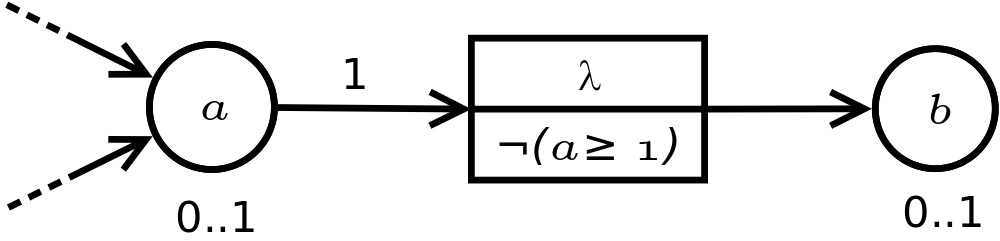
\includegraphics[width=7cm]{figs/ex-hoare-rrg}
  \caption{Un graphe d'interaction partiel. On suppose que le gène $b$ n'est influencé que via le multiplexe $\lambda$, mais que le gène $a$ peut être influencé par d'éventuels autres gènes dans le graphe.}
  \label{hoare-ex-hoare-rrg}
\end{figure}

Afin d'illustrer ce nouveau formalisme, considérons le graphe d'interaction de la figure~\ref{hoare-ex-hoare-rrg}. On suppose que d'autres gènes peuvent influer sur $a$, mais pas sur $b$.
On cherche à savoir s'il existe pour ce graphe une paramétrisation qui accepte que $b$ soit incrémenté si le niveau d'expression de $a$ est à $0$. Pour cela, on considérera le triplet de Hoare suivant :
  \hbegin a = 0 \wedge b = 0 \ha b+ \hb b = 1 \hend
On se place ainsi dans une configuration initiale où les niveaux d'expression de $a$ et $b$ sont nuls, et le chemin consiste simplement en une incrémentation de $b$. Ce triplet est intuitivement vérifié (cela sera prouvé par la suite) mais il n'est pas assez expressif. Nous allons donc utiliser l'opérateur de plus faible pré-condition afin d'obtenir des informations sur la paramétrisation nécessaire pour obtenir un tel comportement. Le résultat est la conjonction $R$ suivante :
\begin{listesanspuce}
\item $R \equiv \left\{\begin{array}{l}
  \Phi^+_b\\
  b = 0
\end{array}\right.$
\end{listesanspuce}
Lorsqu'on on décompose $\Phi^+_b$ on obtient :
\begin{listesanspuce}
\item $R \equiv \left\{\begin{array}{l}
  0 \leq b\\
  b < b_b\\
  \Phi^{\emptyset}_b \Rightarrow k_{b, \emptyset} > b\\
  \Phi^{\{\lambda\}}_b \Rightarrow k_{b, \{\lambda\}} > b\\
  b = 0
\end{array}\right.$
\end{listesanspuce}
Comme le multiplexe $\lambda$ est le seul prédécesseur de $b$, $\Phi^{\emptyset}_b$ et $\Phi^{\{\lambda\}}_b$ s'écriront uniquement en fonction de l'assertion portée par $\lambda$. Comme $\Phi^{\{\lambda\}}_b$ caractérise le cas où l'assertion de $\lambda$ est satisfaite, et $\Phi^{\emptyset}_b$ caractérise le cas contraire, on a :
\begin{listesanspuce}
  \item $\begin{array}{llrlr}
  \Phi^{\{\lambda\}}_b &\equiv& \varphi_{\lambda} &\equiv& \neg (a \geq 1)\\
  \Phi^{\emptyset}_b &\equiv& \neg \varphi_{\lambda} &\equiv& \neg\neg (a \geq 1)
\end{array}$
\end{listesanspuce}
On obtient donc en remplaçant et après simplification :
\begin{listesanspuce}
\item $R \equiv \left\{\begin{array}{l}
  b = 0\\
  (a = 1) \Rightarrow k_{b, \emptyset} > 0\\
  (a = 0) \Rightarrow k_{b, \{\lambda\}} > 0\\
\end{array}\right.$
\end{listesanspuce}
Ce résultat traduit le fait que si on souhaite incrémenter $b$ lorsque son niveau d'expression est nul, alors sa paramétrisation associée ne doit pas être égale à zéro. On retrouve donc l'une des propriétés intrinsèques au modèle de Thomas.

On peut tout d'abord constater que le triplet de départ \hbegini a = 0 \wedge b = 0 \ha b+ \hb b = 1 \hendi{} était effectivement correct, car on a bien :
\begin{listesanspuce}
  \item $a = 0 \wedge b = 0 \Rightarrow R$
\end{listesanspuce}
De plus, on peut extraire de $R$ l'information recherchée : en effet, si on suppose $a$ nul à l'état initial, on trouve la condition nécessaire suivante sur la paramétrisation : $k_{b, \{\lambda\}} > 0$.\\

Ce cas volontairement très simple illustre le fonctionnement de ce croisement entre formalismes. Il permet d'obtenir des conditions sur des cas plus complexes, mais permet aussi de déterminer le caractère réalisable ou non d'un chemin. Par exemple, le chemin $b+ ; b-$ sur le graphe précédent n'est pas possible (du simple fait qu'un autre gène au moins doit exprimer une influence sur $b$ pour que l'évolution de celui-ci puisse changer de direction). En effet, si on suit une démarche similaire (comportant cette fois deux étapes, soit une par instruction), on obtient pour plus faible pré-condition une assertion incohérente, qui caractérise le fait que le programme ne pourra jamais s'exécuter quelle que soit la pré-condition. En revanche, un chemin de type $b+ ; a+ ; b-$ serait envisageable et la méthode présentée donnerait une condition nécessaire sur la paramétrisation pour qu'elle se réalise.





\chapter*{Conclusion}
\addcontentsline{toc}{chapter}{Conclusion}
Dans ce rapport bibliographique a été présenté le modèle de Thomas, qui permet l'étude des systèmes de gènes interagissant entre eux, puis ont été présentées deux techniques d'analyse de ce modèle.

L'étude des interactions génétiques nécessite des outils de modélisation et d'abstraction. Le modèle de Thomas qui a été présenté propose d'approcher un système de gènes en interaction par un réseau de régulation génétique composé d'un graphe d'interactions et d'une paramétrisation. La puissance de ce modèle provient notamment du fait que les niveaux \mbox{d'expression} des gènes y sont représentés par des valeurs discrètes, ce qui permet de prendre uniquement en compte les seuils pour desquels des interactions ont effectivement lieu, mais aussi de s'affranchir de la connaissance des valeurs réelles de ces seuils.

Il est possible à partir de ce type de modèle de construire un graphe d'états qui rend compte de toutes les configurations de niveaux d'expression possibles et des évolutions entre ces configurations. L'approche classique d'étude des graphes d'états consiste en l'utilisation de logiques temporelles. Ces logiques permettent d'exprimer des propriétés sur des états ou des chemins en prenant en compte la dynamique modélisée par le graphe. Dans le cadre du modèle de Thomas, ces logiques permettent d'exprimer des propriétés sur l'évolution d'un réseau de régulation génétique à partir d'un ensemble d'états.

Un nouvel outil d'analyse des réseaux de régulation génétique a enfin été proposé, basé sur la logique de Hoare. Cette logique permet de caractériser un programme à partir d'une pré-condition et d'une post-condition. Rattachée au modèle de Thomas elle permet, \textit{via} l'utilisation de règles d'inférence et de l'opérateur de plus faible pré-condition, d'obtenir par exemple des conditions nécessaires à ce qu'un système de gènes puisse permettre un comportement donné.\\

Le présent séminaire bibliographique a permis le développement des notions qui seront utilisées lors du stage d'application du Master Recherche. La première partie de ce stage consistera en la conception et en l'implémentation informatique du concept de logique de Hoare appliquée aux réseaux de régulation génétique avec multiplexes. Une seconde partie consistera ensuite à enrichir ce concept nouveau et son implémentation en tentant d'ajouter une composante temporelle aux triplets de Hoare utilisés.


\newpage
\addcontentsline{toc}{chapter}{Bibliographie}
\bibliographystyle{abbrv}
\bibliography{biblio}

\end{document}
